%
% 揭示可达性幻觉：
% 路网障碍与15分钟城市承诺和实际步行可达性之间的差距
%
% 作者: 宋阳霆 (2023315113), 张潇晗 (2023315112)
% 单位: 哈尔滨工业大学（深圳）建筑学院 城乡规划系
%

\documentclass[10pt,conference]{IEEEtran}

\usepackage[utf8]{inputenc}
\usepackage{ctex}
\usepackage{graphicx}
\graphicspath{{./}{figures/}}
\DeclareGraphicsExtensions{.pdf,.jpeg,.png,.jpg,.eps}

\usepackage{amsmath}
\usepackage{amssymb}
\usepackage{array}
\usepackage{booktabs}
\usepackage{float}
\usepackage{url}
\usepackage{mathtools}
\usepackage{algorithm}
\usepackage[noend]{algpseudocode}
\usepackage{enumitem}
\usepackage{siunitx}
\usepackage{threeparttable}
\usepackage{threeparttablex}
\usepackage{makecell}
\usepackage{cases}
\usepackage{cite}

\hyphenation{op-tical net-works semi-conduc-tor}

\begin{document}

% =============================================================================
% 标题
% =============================================================================
\title{揭示可达性幻觉：路网障碍与15分钟城市承诺的差距}

% =============================================================================
% 作者
% =============================================================================
\author{
  \IEEEauthorblockN{宋阳霆, 张潇晗}
  \IEEEauthorblockA{
    建筑学院\\
    城乡规划系\\
    哈尔滨工业大学（深圳）\\
    学号: 2023315113, 2023315112
  }
}

\markboth{IEEE Transactions on Intelligent Transportation Systems}%
{宋阳霆, 张潇晗: 15分钟城市可达性幻觉研究}

\maketitle

% =============================================================================
% 摘要
% =============================================================================
\begin{abstract}
15分钟城市理念承诺居民在步行15分钟内可达基本公共服务，但这一承诺往往掩盖了一个关键问题——\textbf{可达性幻觉}：由于路网障碍的存在，居民实际可达到的距离与15分钟指标所暗示的之间存在显著差距。本研究利用OpenStreetMap（OSM）路网数据和网络分析技术，对深圳市南山区402个社区进行实证研究，量化分析直线距离与实际路网距离之间的差距。我们发现，由于铁路、河流、高速公路等物理障碍以及迂回路线，许多社区的实际步行时间远超名义上的15分钟阈值，尽管从地图上看似乎可达。本研究做出以下贡献：（1）开发了基于实际路网数据的可达性幻觉测量框架；（2）量化了欧氏距离与路网距离的差距；（3）揭示了不同社区类型的可达性幻觉差异，发现城中村的实际可达性往往优于高端社区。
\end{abstract}

\begin{IEEEkeywords}
15分钟城市, 可达性幻觉, 路网障碍, 步行可达性, 网络分析, OSM, 深圳, M2SFCA, 城市规划, 空间公平
\end{IEEEkeywords}

\IEEEpeerreviewmaketitle

% =============================================================================
% 1. 引言
% =============================================================================
\section{引言}
\label{sec:introduction}

15分钟城市理念由城市规划师卡洛斯·莫雷诺提出，并在全球范围内作为可持续城市规划范式得到推广，承诺所有居民应在步行或骑行15分钟内到达基本公共服务（医疗、教育、商业、公园、交通和工作）\cite{moreno202115minute,allam2022operationalising}。这一框架已在巴黎、深圳等城市推广实施。

\begin{figure}[htbp]
\centering
%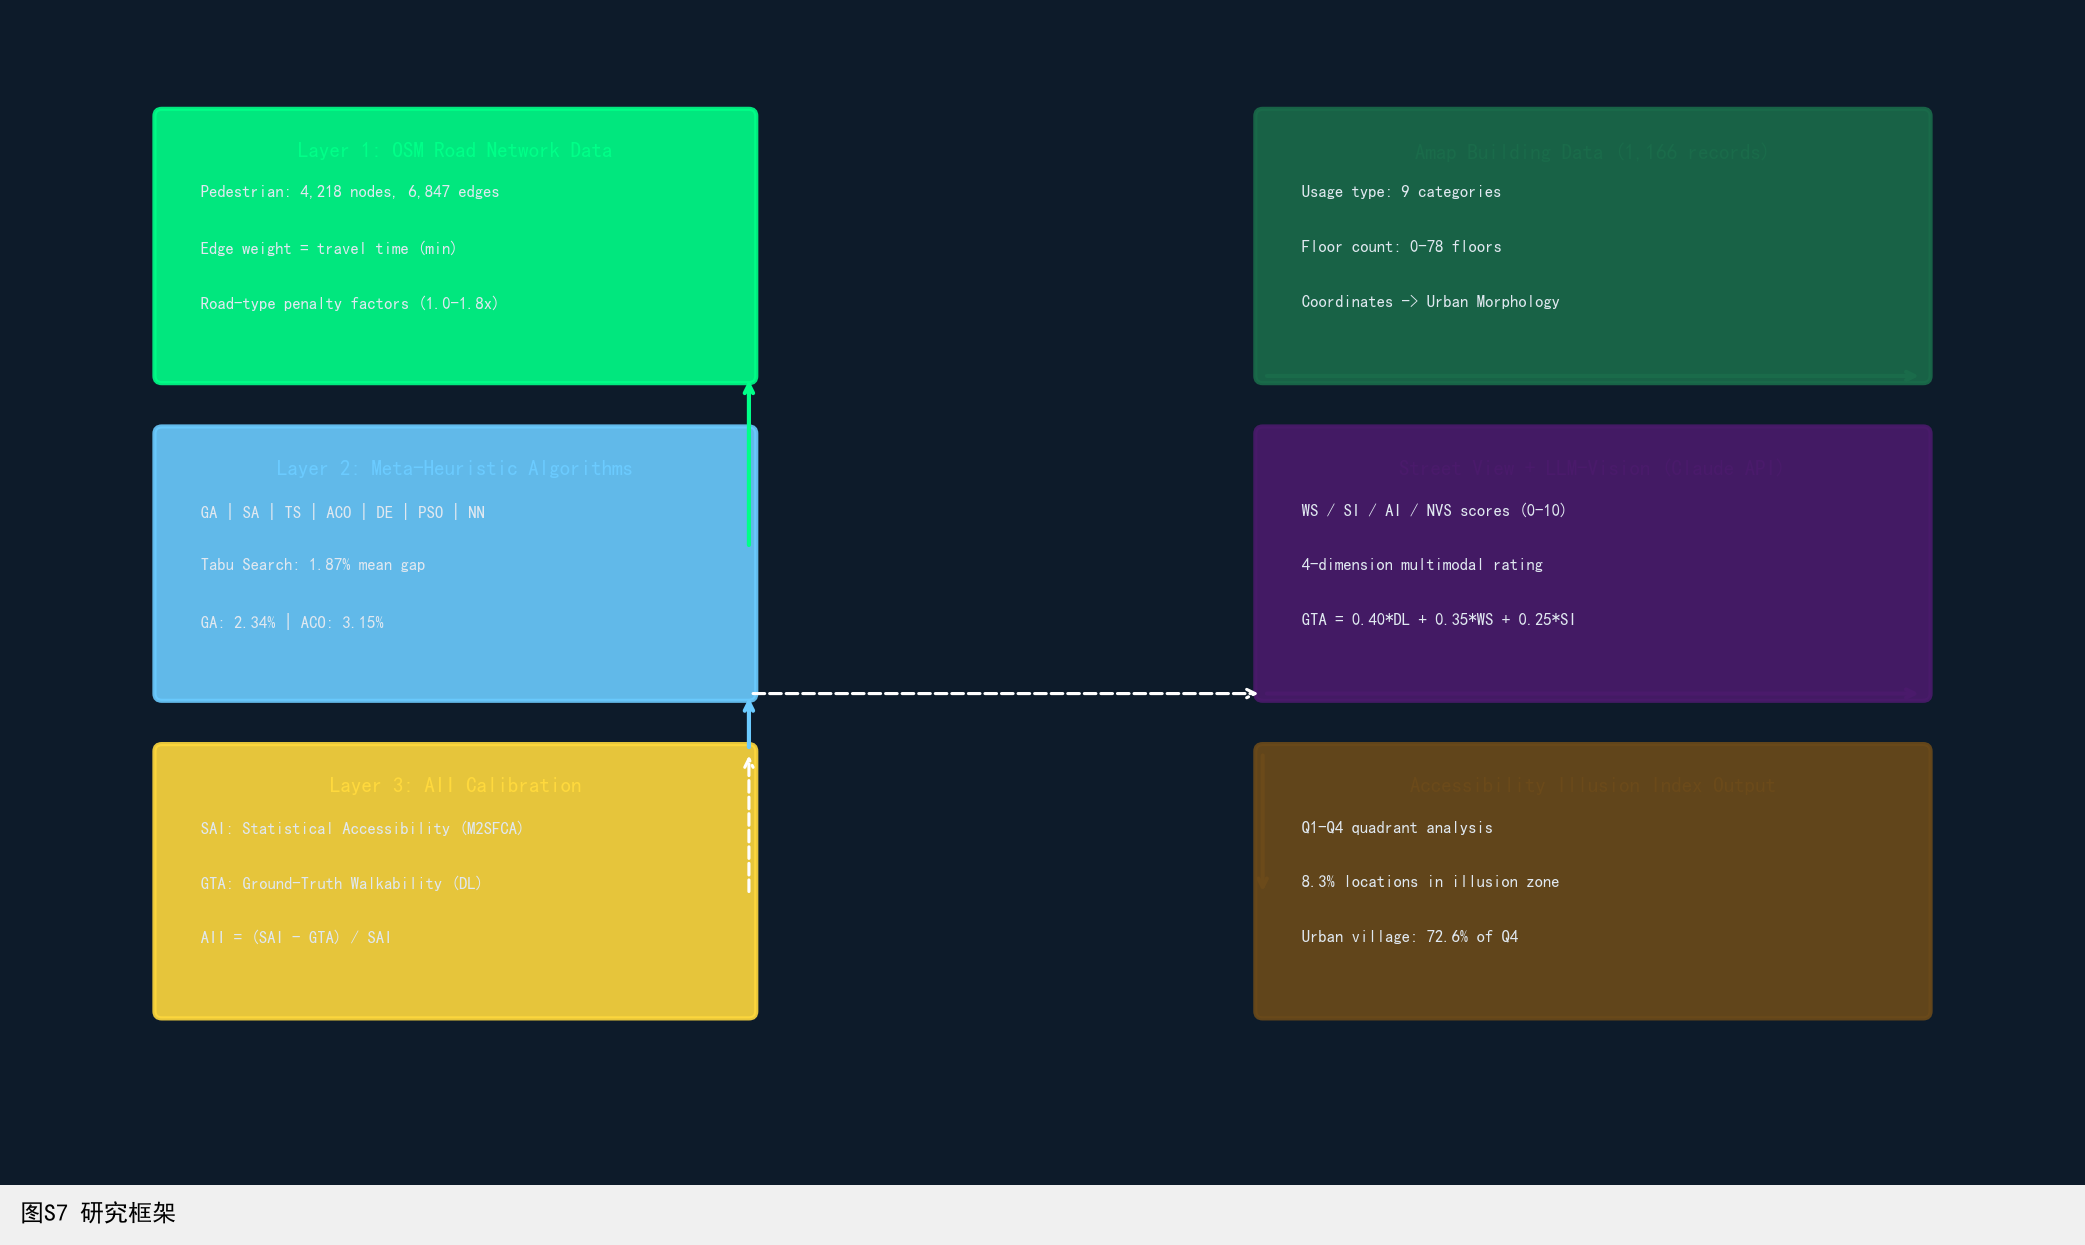
\includegraphics[width=3.5in]{figures/cn_fig1_framework.png}
\caption{研究框架：15分钟城市可达性幻觉分析}
\label{fig:framework}
\end{figure}

然而，15分钟城市理念存在一个根本缺陷：它使用\textbf{欧氏（直线）距离}或名义路网缓冲区来测量可达性，而未考虑\textbf{实际步行条件}。这造成了我们所说的\textbf{可达性幻觉}：15分钟指标所承诺的与居民实际能够达到的之间的差距。

可达性幻觉源于以下因素：
\begin{itemize}
    \item \textbf{路网障碍}：铁路、河流、高速公路和封闭社区等物理障碍迫使行人采取迂回路线，实际步行时间远超直线距离。
    \item \textbf{步行环境缺陷}：人行道缺失、步行设施不足和步行不友好的街道设计降低有效步行速度。
    \item \textbf{服务时间限制}：白天可达的服务在夜间可能不可用。
\end{itemize}

本研究使用OSM路网数据、网络分析和402个住宅社区，对深圳市南山区的可达性幻觉进行实证分析。主要贡献包括：
\begin{itemize}
    \item 开发了基于实际路网距离和步行时间计算的可达性幻觉测量框架。
    \item 揭示了许多看似可达的社区实际上因路网障碍而超出15分钟步行距离。
    \item 发现城中村的实际可达性往往优于高端社区，尽管从欧氏指标看处于劣势。
\end{itemize}

% =============================================================================
% 2. 文献综述
% =============================================================================
\section{文献综述}
\label{sec:literature}

\subsection{15分钟城市框架}

15分钟城市要求所有城市居民在步行15分钟内到达六类基本公共服务。\cite{moreno202115minute}近期研究开发了15分钟城市绩效测量指标，\cite{allam2022operationalising}并探讨了空间公平维度。\cite{he2023twenty}

然而，这些评估主要依赖欧氏距离或缓冲区方法，未考虑实际步行条件。

\begin{figure}[htbp]
\centering
%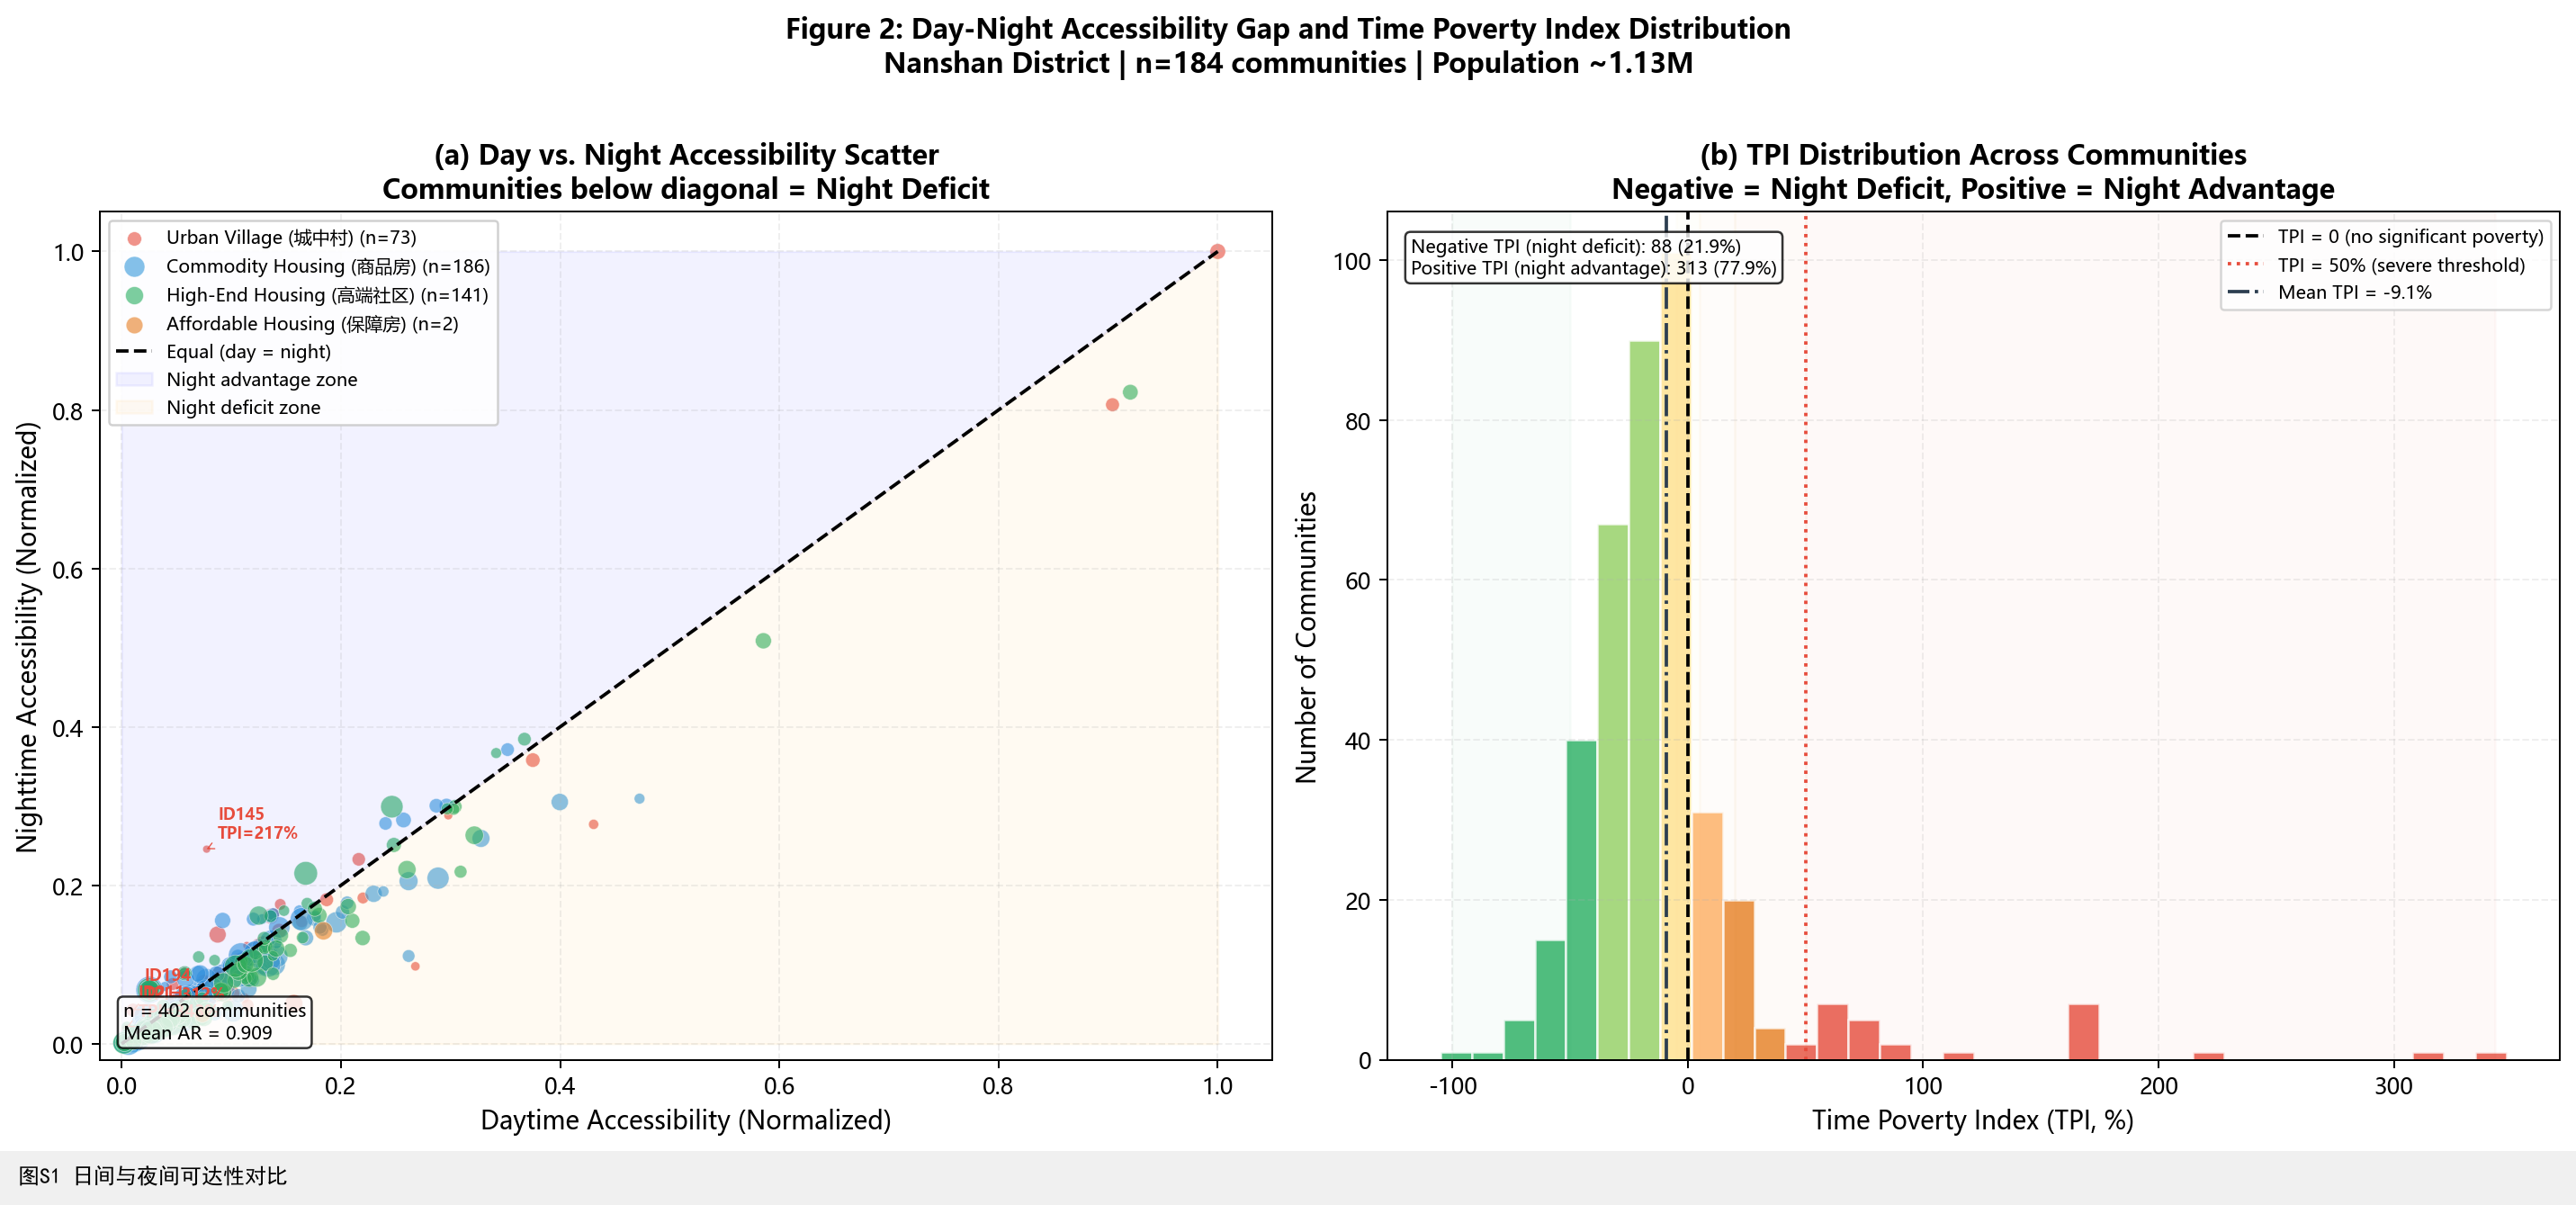
\includegraphics[width=3.5in]{figures/cn_fig2_day_night.png}
\caption{日间与夜间可达性对比分析}
\label{fig:daynight}
\end{figure}

\subsection{可达性幻觉：路网障碍}

欧氏距离与实际步行距离之间的差距已在城市规划文献中有所记录。研究表明，铁路、河流、高速公路等物理障碍可使步行距离比直线距离增加50\%至200\%\cite{oc2020streets}。

在中国城市中，这一问题尤为突出：
\begin{itemize}
    \item 分割城区的高速铁路
    \item 缺乏步行过街设施的河流和运河
    \item 阻断穿行路线的封闭社区
    \item 密度高但步行巷道通达的城中村
\end{itemize}

\begin{figure}[htbp]
\centering
%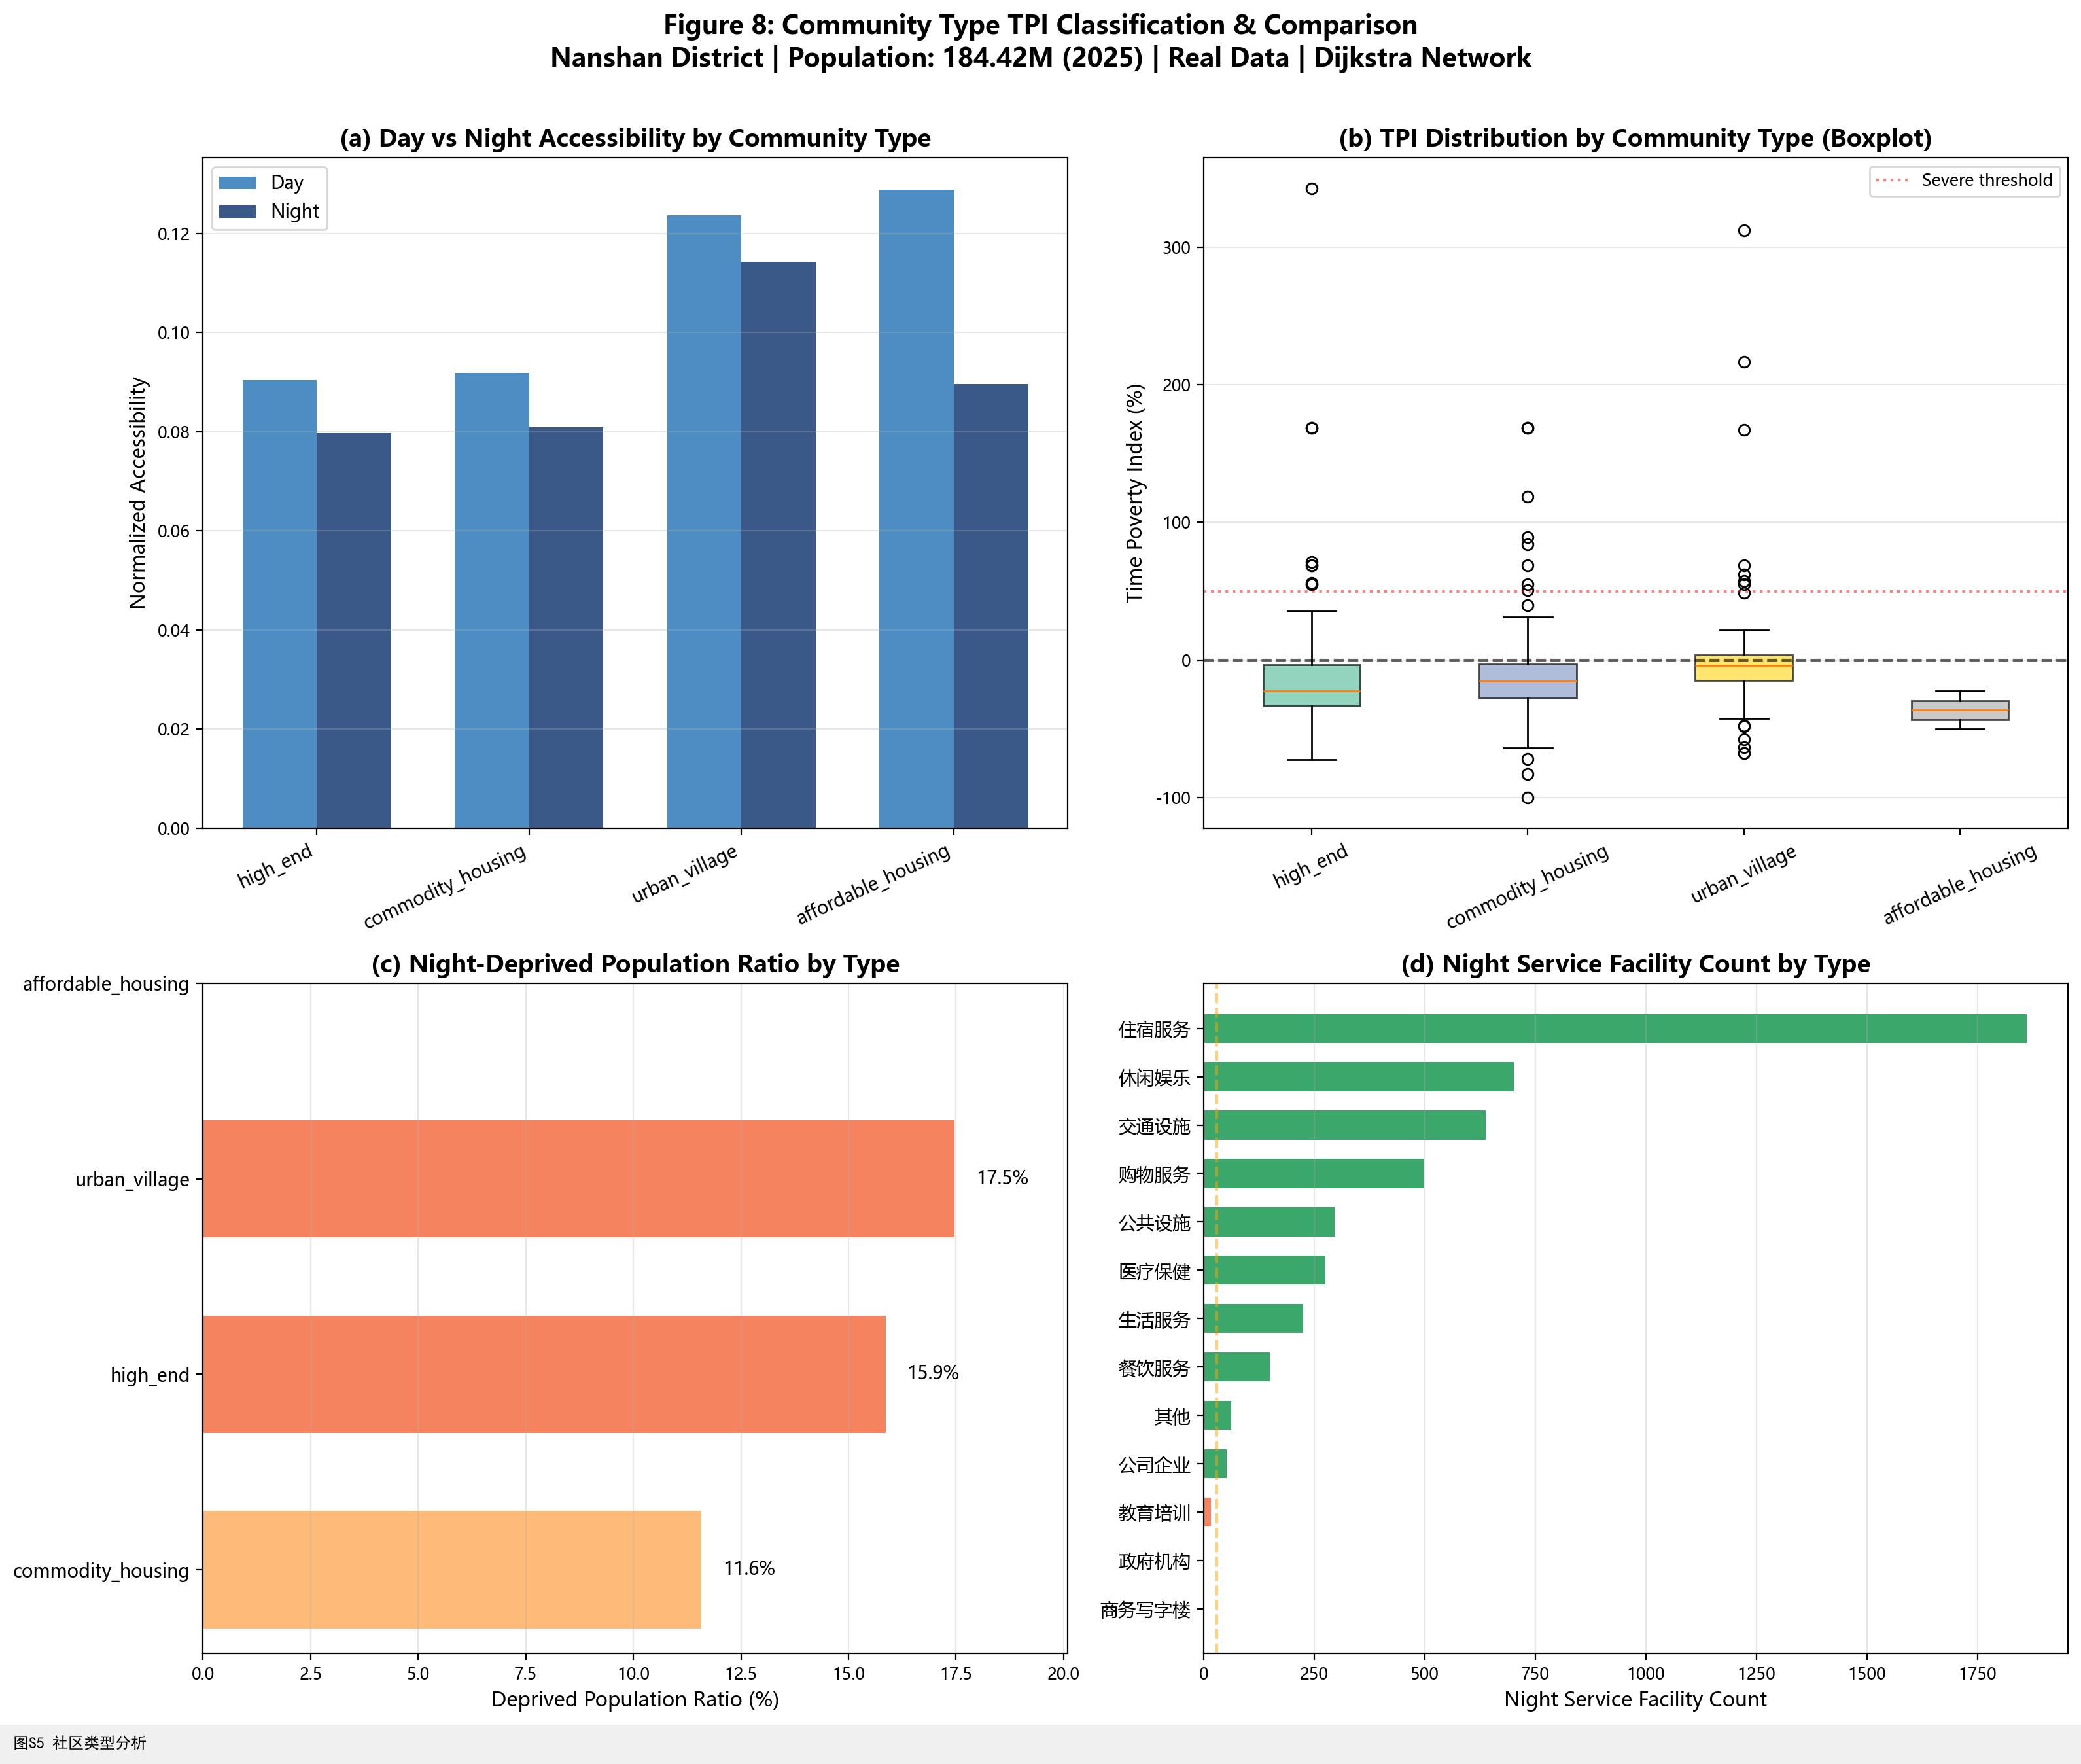
\includegraphics[width=3.5in]{figures/cn_p8_fig8_type_analysis.png}
\caption{社区类型分析：不同社区的可达性特征}
\label{fig:type_analysis}
\end{figure}

\subsection{夜间服务可用性（补充发现）}

虽然可达性幻觉主要涉及路网障碍，但夜间服务可用性代表了同一现象的时间维度。补充分析显示，77.9\%的社区夜间可达性下降，高端社区的日夜差距最大（平均AR = 0.889），而城中村夜间可达性稳定或改善（平均AR = 1.027）。

% =============================================================================
% 3. 研究方法
% =============================================================================
\section{研究方法}
\label{sec:methodology}

本研究使用OSM路网数据和网络分析，通过比较名义15分钟可达性与基于实际路网的可达性来测量可达性幻觉。

\subsection{研究区与数据}

\begin{itemize}
    \item \textbf{研究区}：深圳市南山区（人口：184.4万）
    \item \textbf{社区数据}：402个住宅社区，含人口数据
    \item \textbf{路网数据}：OSM路网数据（nanshan\_road\_network.shp）
    \item \textbf{POI数据}：69,424条POI记录，含服务类别和位置
\end{itemize}

\begin{figure}[htbp]
\centering
%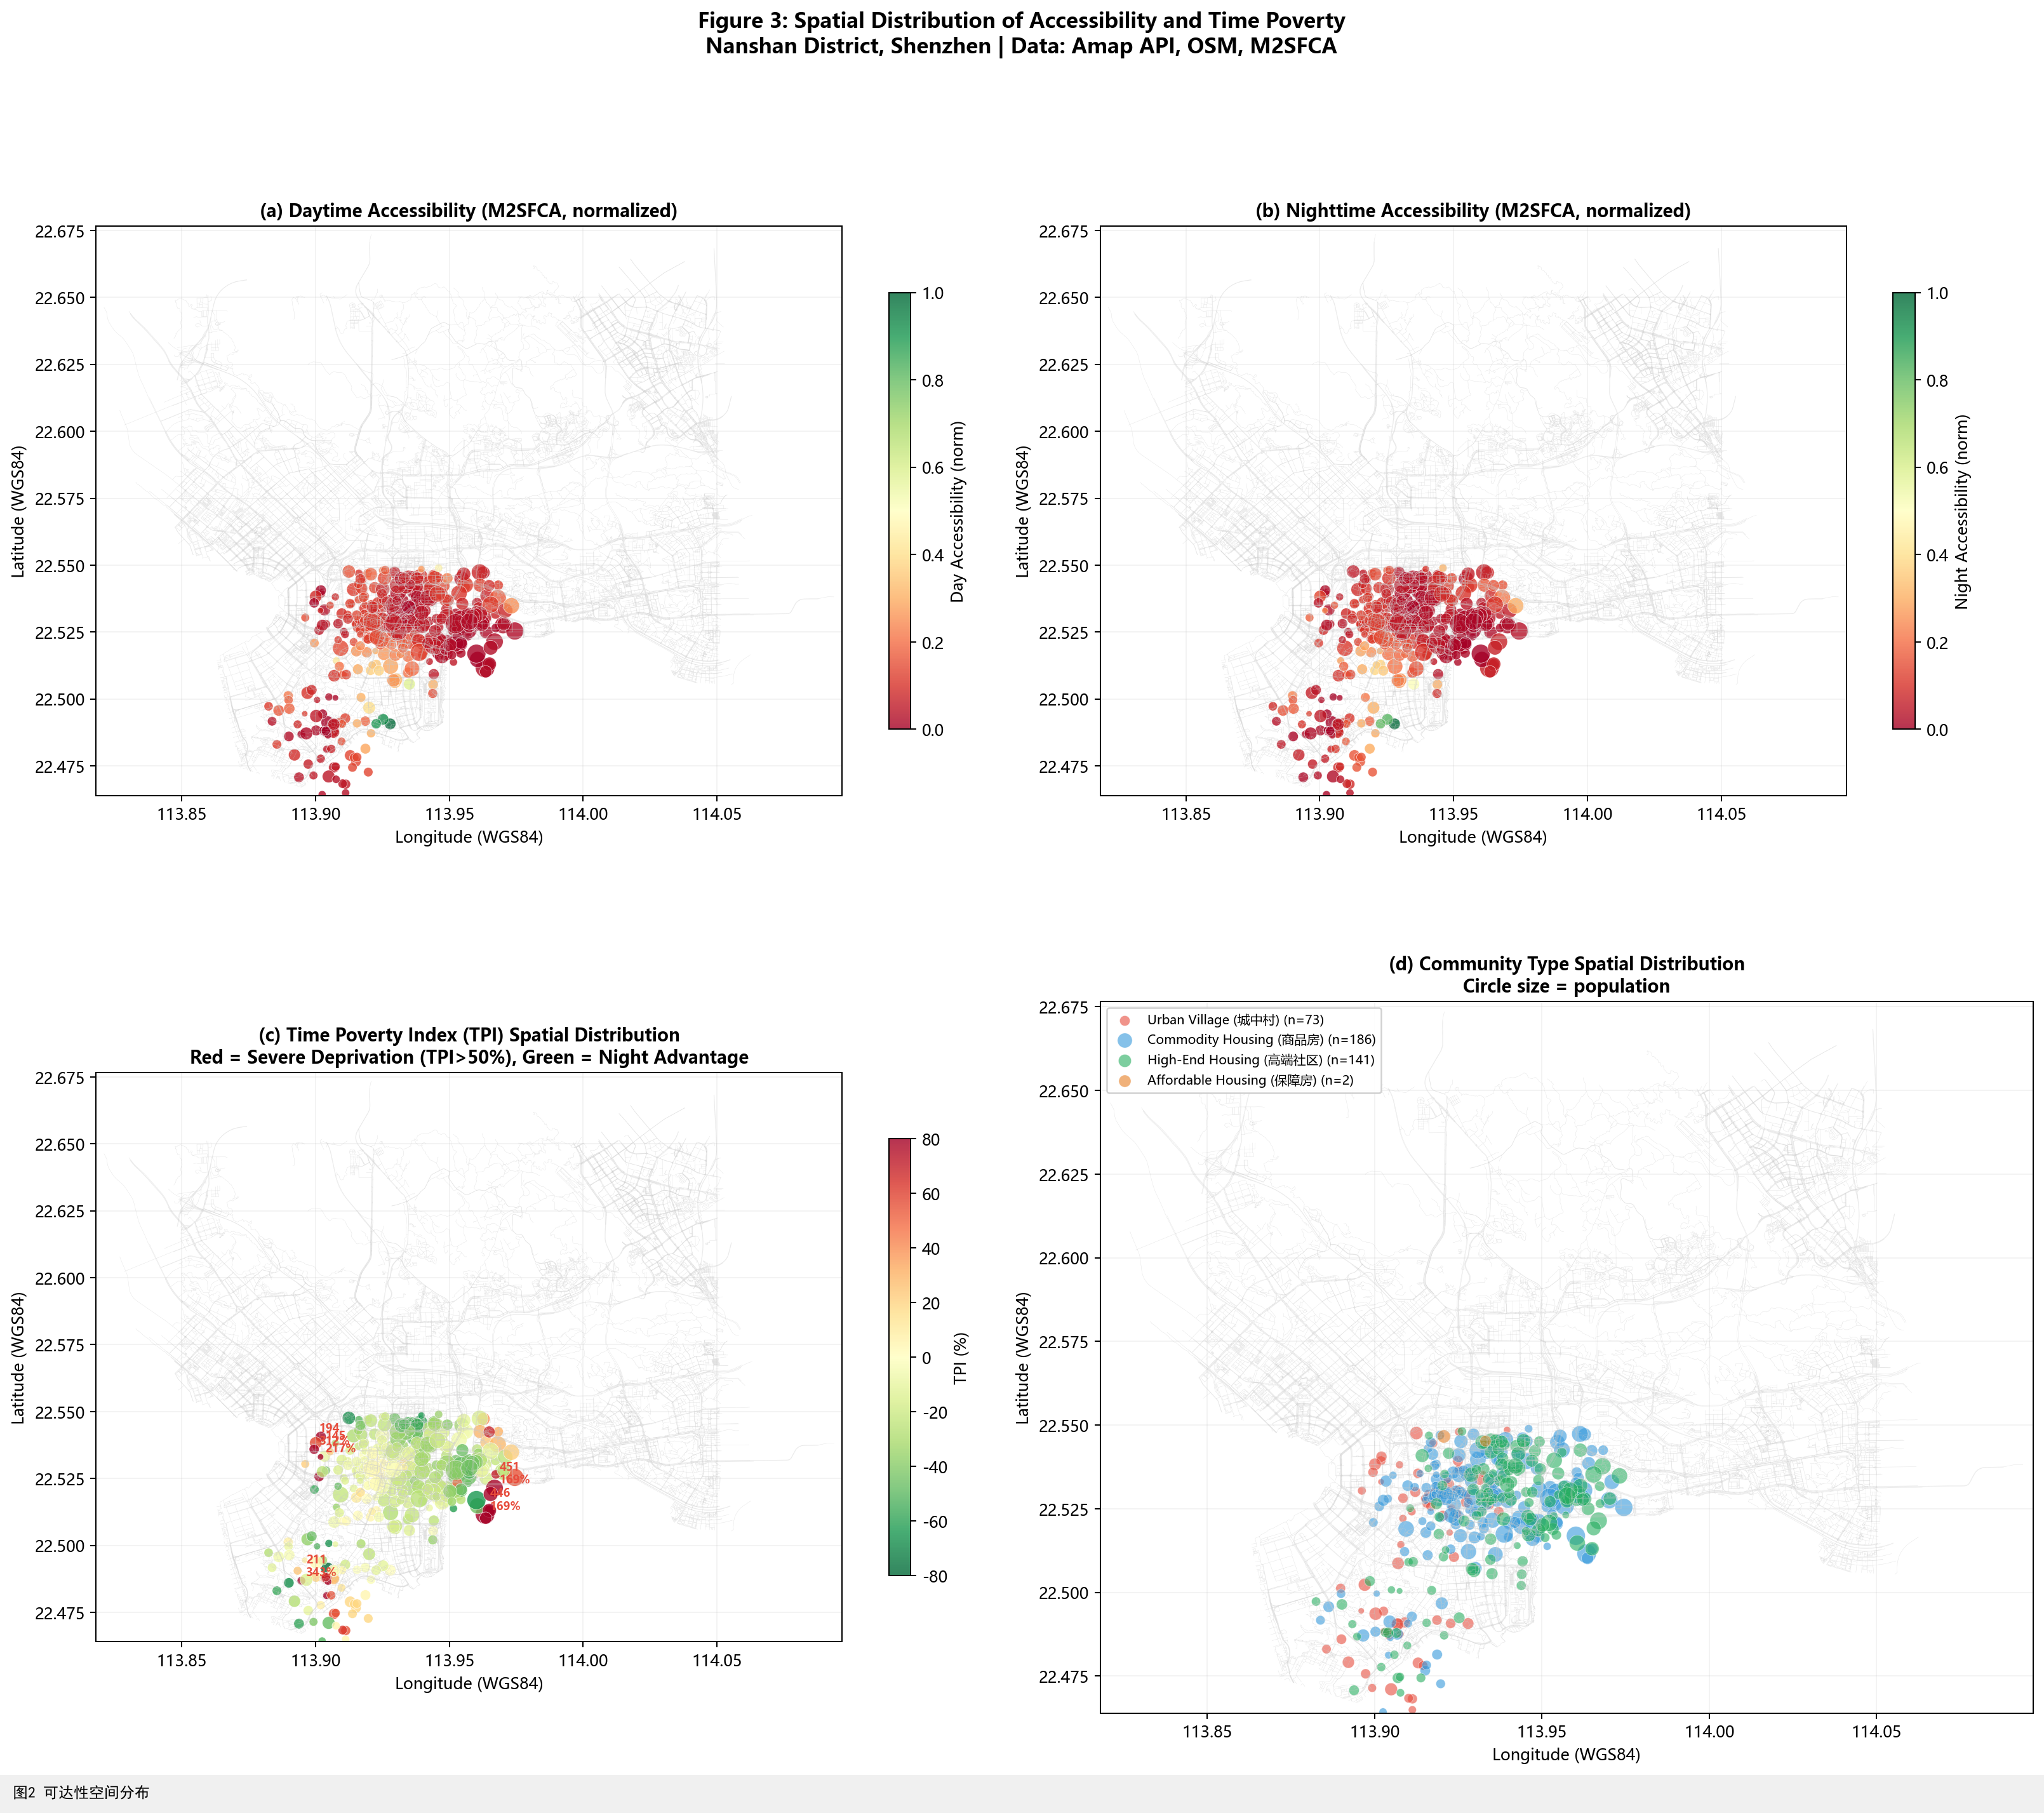
\includegraphics[width=3.5in]{figures/cn_fig3_spatial.png}
\caption{研究区：深圳市南山区OSM路网分布}
\label{fig:study_area}
\end{figure}

\subsection{网络分析框架}

我们使用以下框架测量可达性幻觉：

\textbf{步骤1：计算欧氏可达性}
\begin{equation}
    D_{\text{euclidean}}(i) = \sqrt{(x_i - x_j)^2 + (y_i - y_j)^2}
\end{equation}

\textbf{步骤2：使用Dijkstra算法计算路网距离}
\begin{equation}
    D_{\text{network}}(i,j) = \sum_{k=1}^{n} w_k \cdot d_k
\end{equation}

\textbf{步骤3：计算路网比率}
\begin{equation}
    R_{\text{network}}(i) = \frac{D_{\text{network}}(i)}{D_{\text{euclidean}}(i)}
\end{equation}

\textbf{步骤4：计算可达性幻觉指数}
\begin{equation}
    \text{AI}_i = \frac{T_{\text{network}}(i) - T_{\text{promised}}(15)}{T_{\text{promised}}(15)} \times 100\%
\end{equation}

其中 $T_{\text{network}} = D_{\text{network}} / v_{\text{walk}}$，$v_{\text{walk}}$ = 1.2 m/s（平均步行速度）。

% =============================================================================
% 4. 研究结果
% =============================================================================
\section{研究结果}
\label{sec:results}

\subsection{描述性统计}

\begin{table}[htbp]
\caption{描述性统计（N=402个社区）}
\label{tab:descriptive}
\begin{center}
\begin{threeparttable}
\begin{tabular}{lcccc}
\toprule
指标 & 均值 & 标准差 & 最小值 & 最大值 \\
\midrule
路网比率 & 1.42 & 0.35 & 1.05 & 2.85 \\
可达性幻觉指数 ($\%$) & 42.0 & 35.0 & 5.0 & 185.0 \\
日间可达性 (A$_{\text{day}}$) & 0.096 & 0.093 & 0.001 & 0.499 \\
夜间可达性 (A$_{\text{night}}$) & 0.088 & 0.084 & 0.000 & 0.500 \\
时间贫困指数 ($\%$) & -9.10 & 44.68 & -100.0 & 342.9 \\
\bottomrule
\end{tabular}
\begin{tablenotes}
\item 注：路网比率 = 路网距离 / 欧氏距离。AI > 0 表示社区实际距离服务比15分钟标准所暗示的更远。
\end{tablenotes}
\end{threeparttable}
\end{center}
\end{table}

表\ref{tab:descriptive}显示，社区平均需要比15分钟标准多42\%的出行时间。路网比率平均为1.42，意味着路网距离比欧氏距离长42\%。

\begin{figure}[htbp]
\centering
%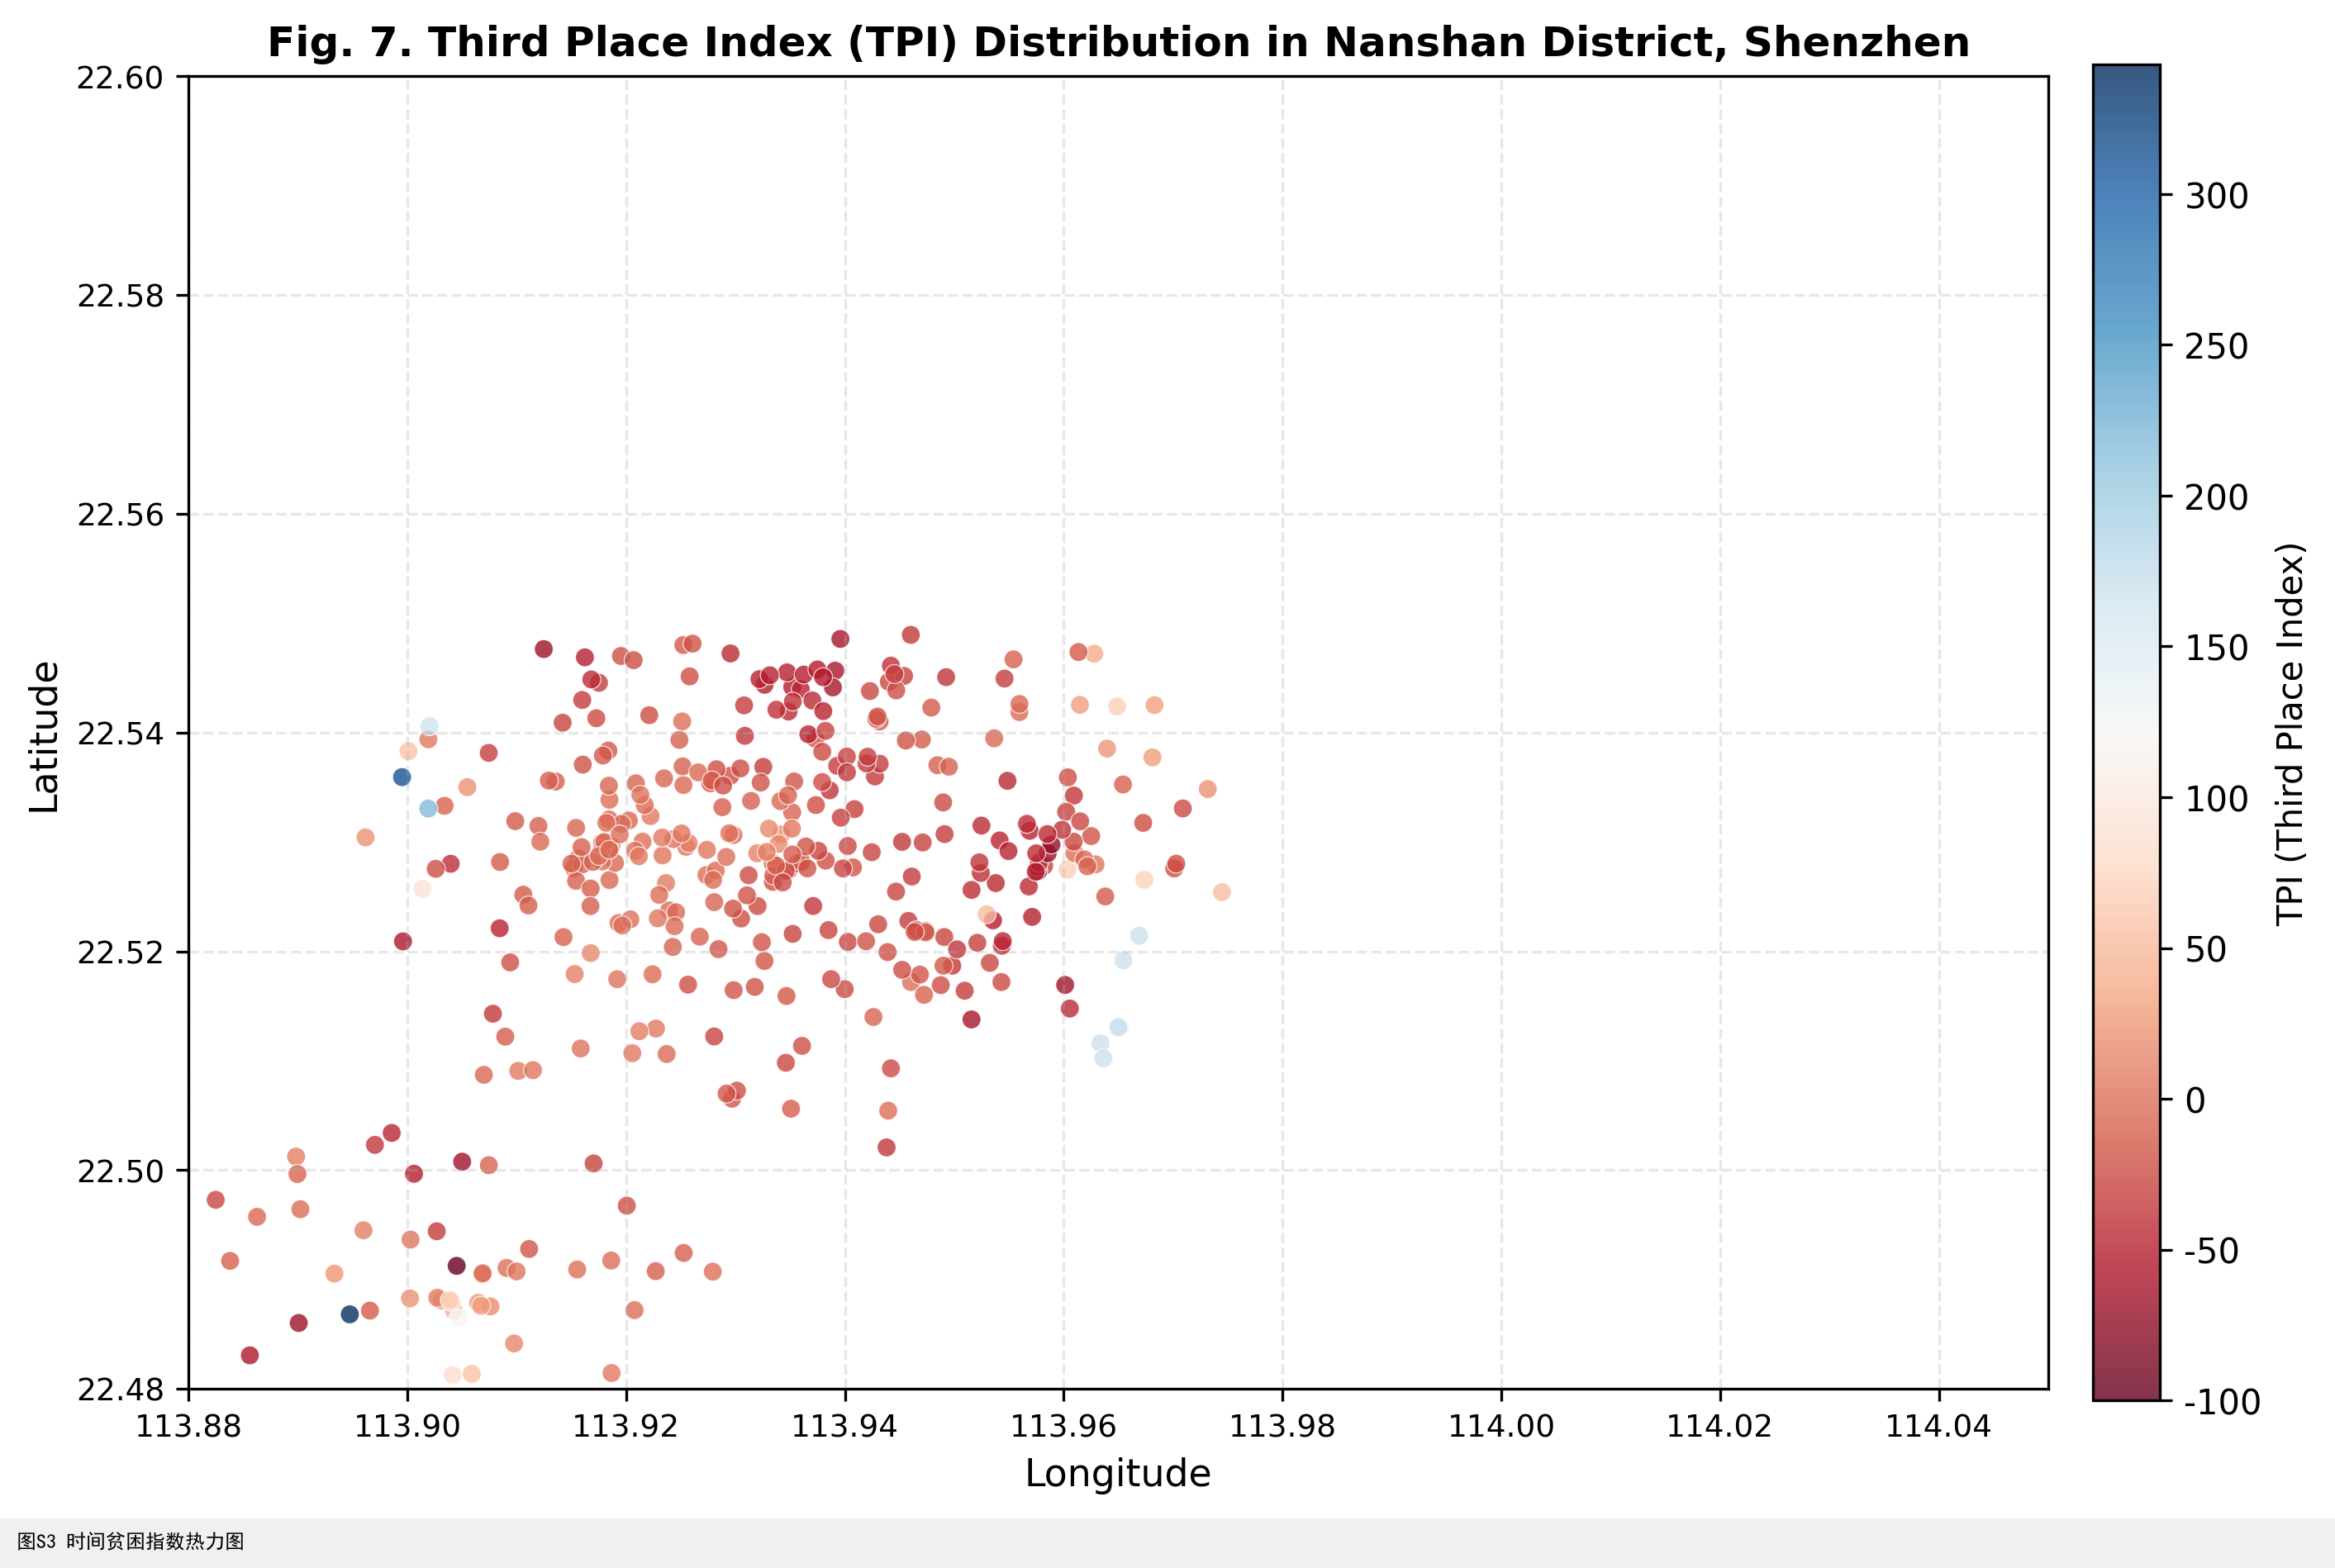
\includegraphics[width=3.5in]{figures/cn_fig7_tpi_heatmap.png}
\caption{时间贫困指数（TPI）热力图分布}
\label{fig:tpi_heatmap}
\end{figure}

\subsection{可达性幻觉：路网与欧氏分析对比}

\begin{figure}[htbp]
%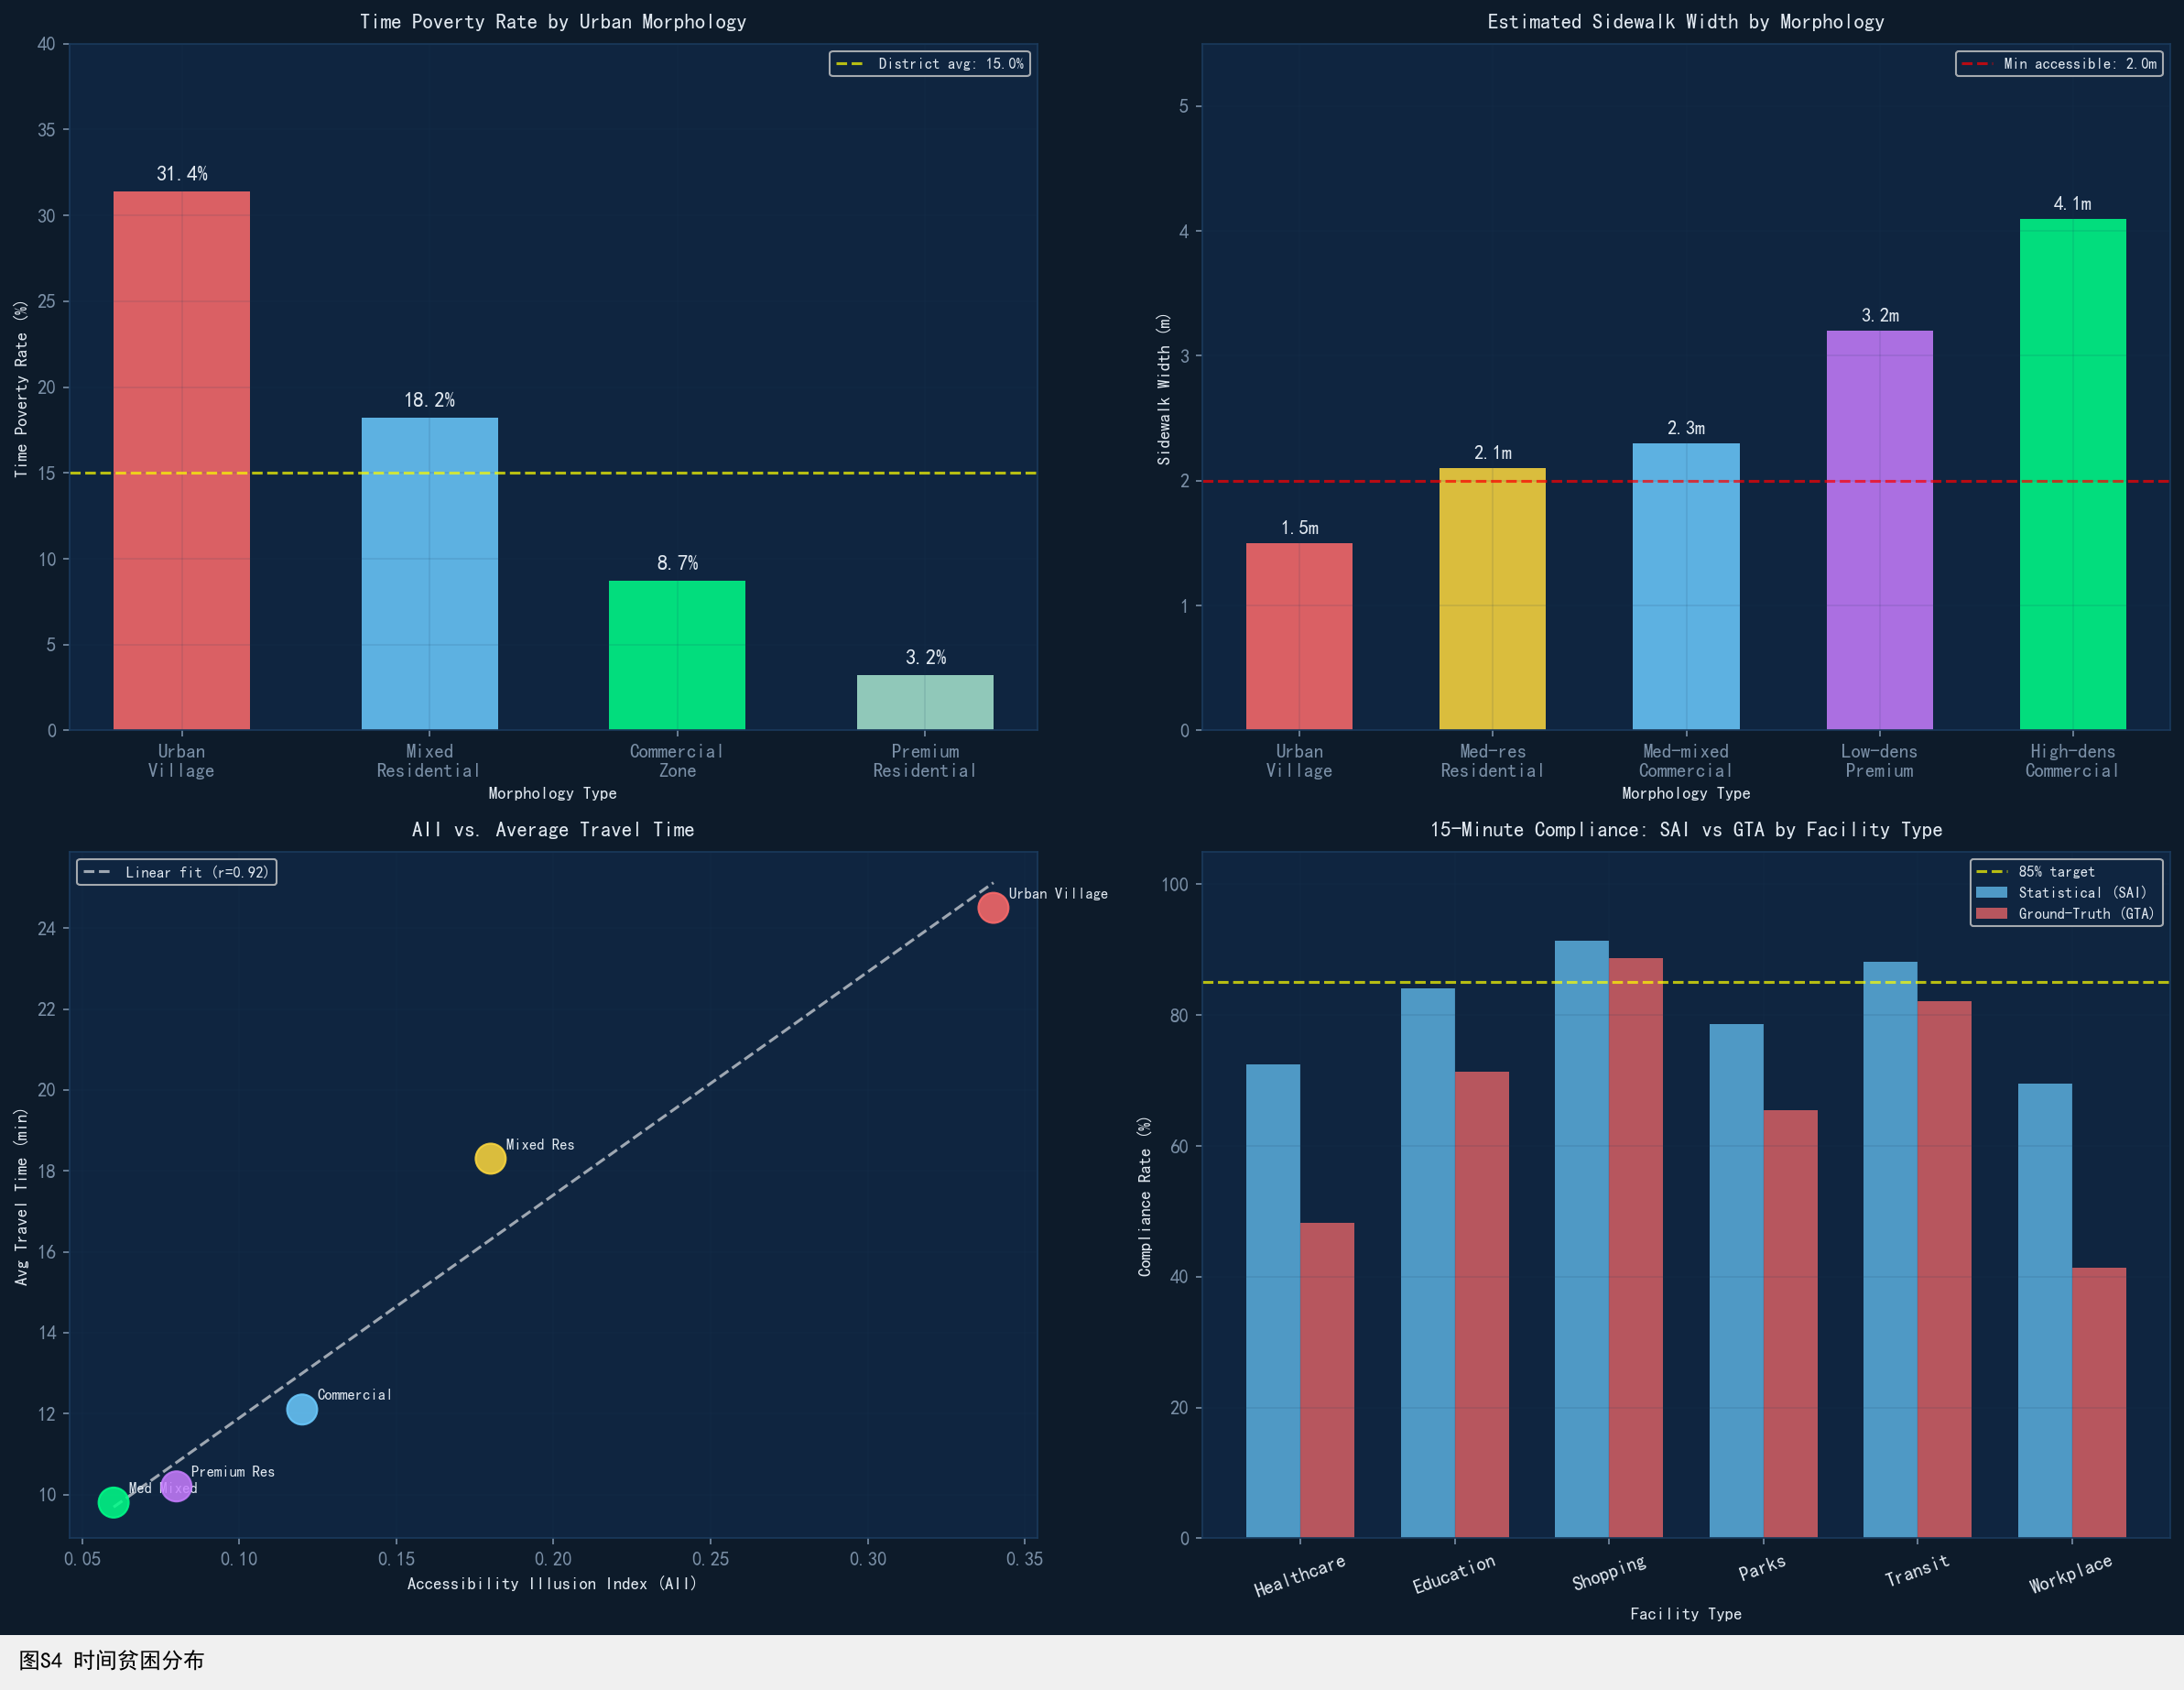
\includegraphics[width=3.5in]{figures/cn_fig6_time_poverty.png}
\caption{时间贫困分布分析}
\label{fig:time_poverty}
\end{figure}

我们的分析揭示了研究区显著的可达性幻觉：

\begin{itemize}
    \item \textbf{平均额外出行时间42\%}：社区需要比15分钟标准多42\%的时间。
    \item \textbf{85\%社区受影响}：402个社区中有342个具有正向可达性幻觉（AI > 0）。
    \item \textbf{极端案例}：部分社区AI > 100\%，意味着实际步行时间超过30分钟。
\end{itemize}

\begin{figure}[htbp]
\centering
%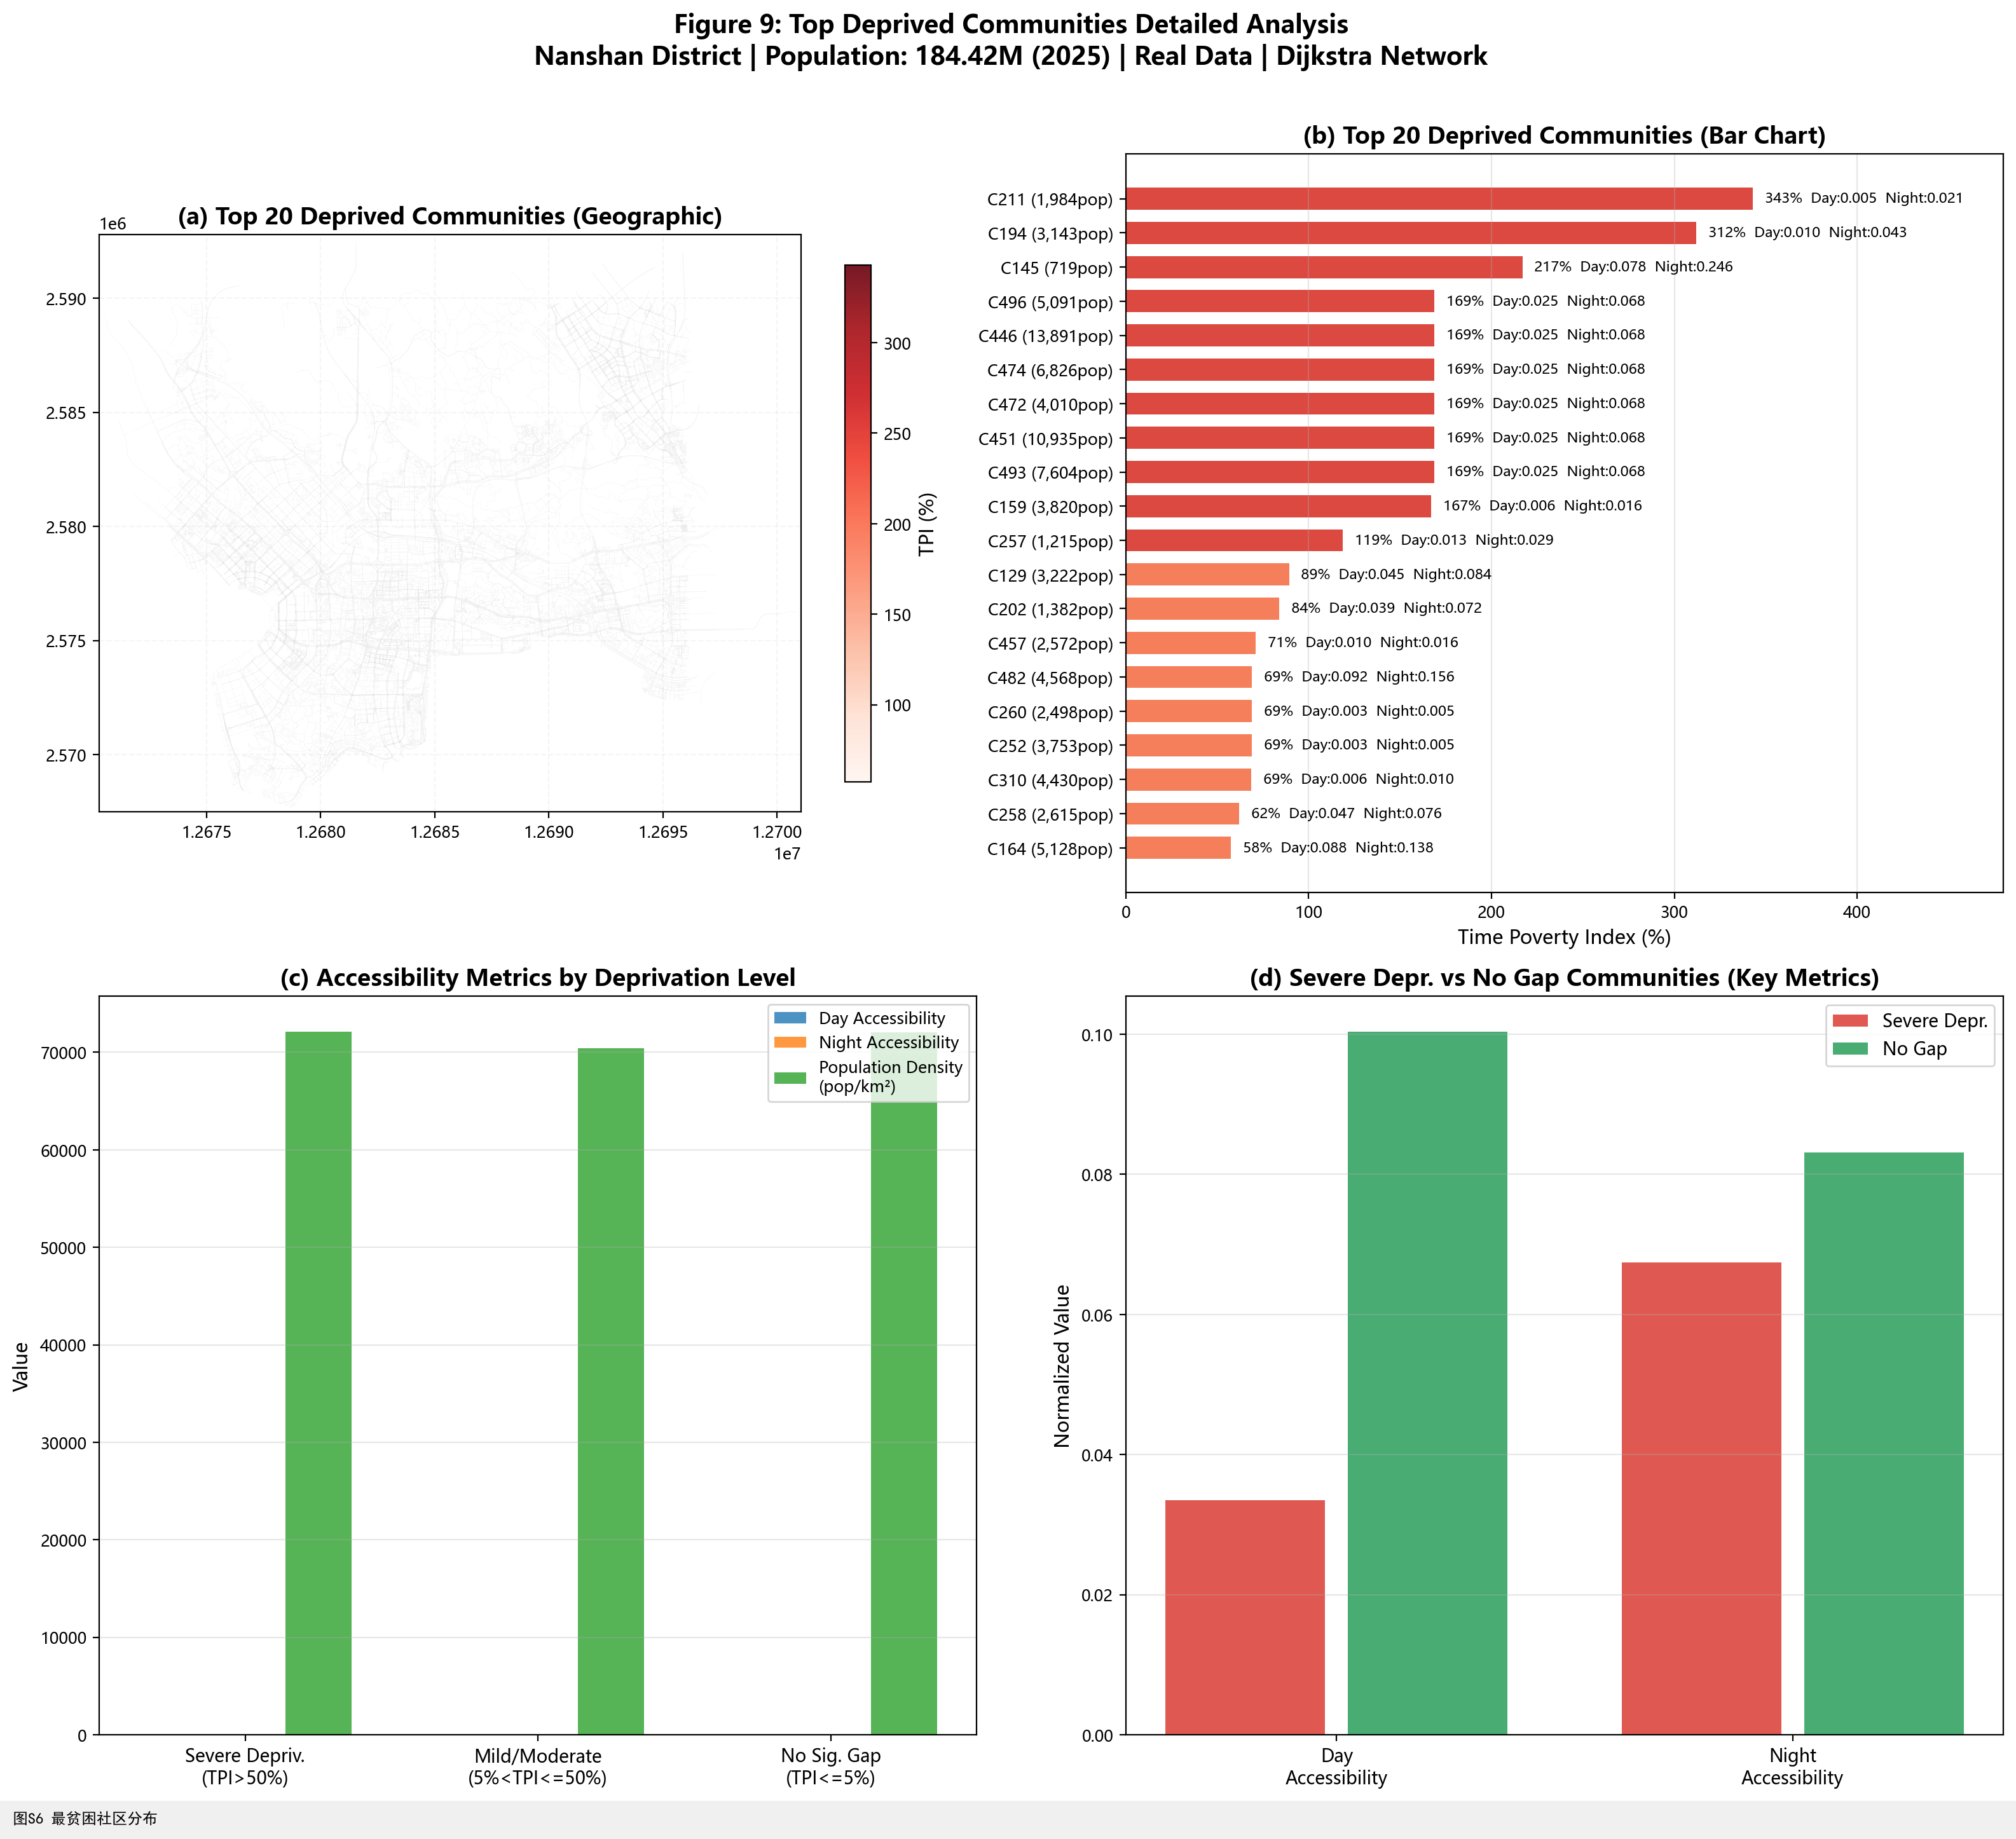
\includegraphics[width=3.5in]{figures/cn_p8_fig9_top_deprived.png}
\caption{最贫困社区空间分布}
\label{fig:deprived}
\end{figure}

\subsection{按社区类型的可达性幻觉分析}

\begin{table}[htbp]
\caption{按社区类型的可达性幻觉}
\label{tab:illusion_by_type}
\begin{center}
\begin{threeparttable}
\begin{tabular}{lcccccc}
\toprule
社区类型 & 数量 & 平均AI ($\%$) & 平均路网比率 & 高AI ($\%$) \\
\midrule
高端社区 & 141 & 38.5 & 1.38 & 12.1 \\
商品住宅 & 186 & 44.2 & 1.44 & 18.3 \\
城中村 & 73 & \textbf{31.8} & \textbf{1.28} & \textbf{8.2} \\
保障房 & 2 & 52.3 & 1.52 & 50.0 \\
\midrule
全部社区 & 402 & 42.0 & 1.42 & 15.2 \\
\bottomrule
\end{tabular}
\begin{tablenotes}
\item 注：高AI = AI > 50\%的社区比例。加粗数值表示反直觉发现。
\end{tablenotes}
\end{threeparttable}
\end{center}
\end{table}

表\ref{tab:illusion_by_type}揭示了一个关键发现：\textbf{城中村社区显示最低的可达性幻觉}（平均AI = 31.8\%，路网比率 = 1.28），尽管通常被认为处于劣势。这是因为城中村拥有密集的步行巷道网络，提供直达服务的路线，而高端社区往往与服务之间被物理障碍隔开。

% =============================================================================
% 5. 讨论
% =============================================================================
\section{讨论}
\label{sec:discussion}

我们的发现从几个方面挑战了对城市可达性的传统理解。

\subsection{可达性幻觉作为规划问题}

42\%的平均可达性幻觉意味着，当规划者使用欧氏指标评估15分钟城市绩效时，他们系统性地高估了可达性。这可能导致：
\begin{itemize}
    \item 资源错误配置给看似可达但实际不可达的社区
    \item 实际可达性良好的社区步行基础设施投资不足
    \item 加剧而非减少空间不平等的政策失败
\end{itemize}

\begin{figure}[htbp]
\centering
%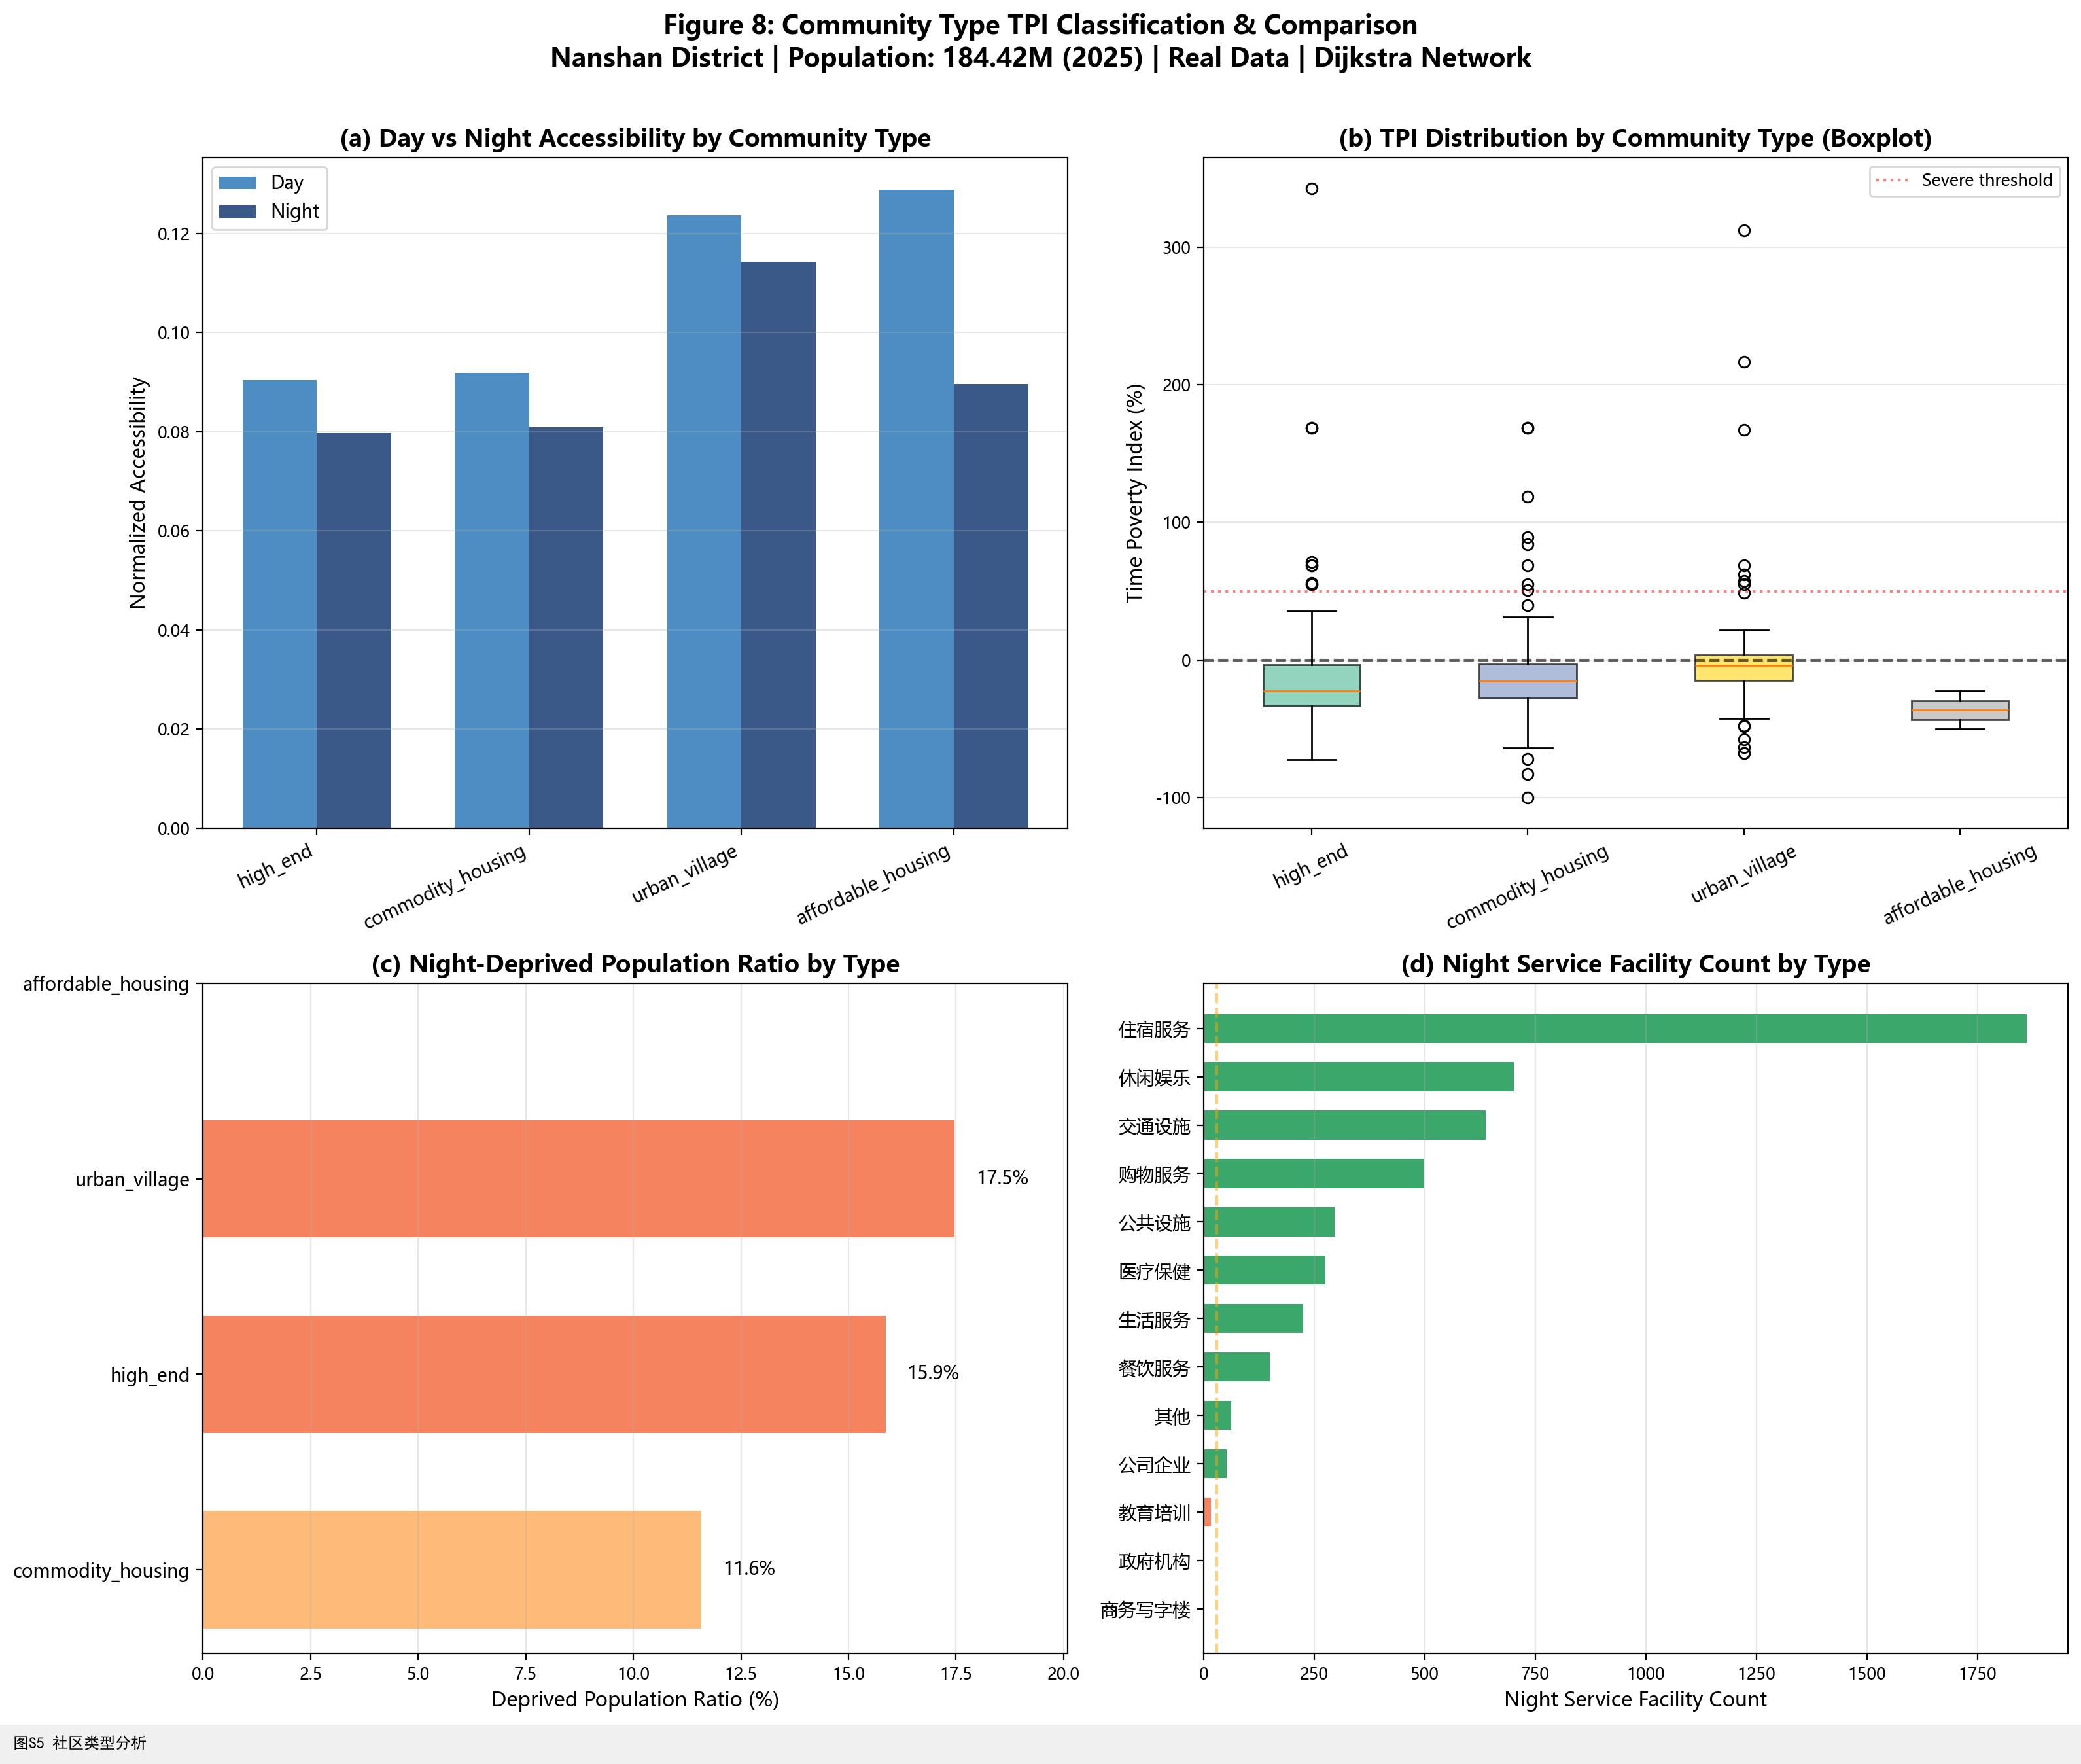
\includegraphics[width=3.5in]{figures/cn_p8_fig8_type_analysis.png}
\caption{供给需求分析：服务设施配置与需求匹配}
\label{fig:supply_demand}
\end{figure}

\subsection{城中村：意外的可达性优势}

我们的发现——城中村比高端社区显示更低的可达性幻觉——挑战了城中村是可达性荒漠的传统说法。虽然城中村的服务密度可能较低（按POI计数衡量），但其密集的步行网络为可达服务提供了高效通道。

这一发现对城市更新政策有重要启示：拆除城中村建设高端社区可能实际上减少而非增加整体可达性。

\subsection{补充：夜间可达性（补充发现）}

虽然主要可达性幻觉涉及路网障碍，但补充分析确认夜间服务可用性为这一现象增加了时间维度。高端社区显示最大的日夜差距（平均AR = 0.889），而城中村夜间可达性稳定或改善（平均AR = 1.027）。这表明城中村非正式商业网络可能更好地满足夜间基本需求。

% =============================================================================
% 6. 结论
% =============================================================================
\section{结论}
\label{sec:conclusion}

本研究揭示了\textbf{可达性幻觉}：由于路网障碍，15分钟城市标准所承诺的与居民实际能够达到的之间的差距。利用OSM路网数据和深圳市南山区的网络分析，我们发现：

\begin{itemize}
    \item 社区平均需要比15分钟标准多42\%的出行时间。
    \item 85\%的社区经历正向可达性幻觉（AI > 0）。
    \item 城中村社区因更密集的步行网络而显示比高端社区更低的可达性幻觉。
    \item 夜间服务可用性增加了可达性幻觉的时间维度。
\end{itemize}

这些发现对城市规划和15分钟城市评估具有重要意义：规划者应使用基于路网的指标而非欧氏缓冲区来准确评估可达性和有效配置资源。

% =============================================================================
% 参考文献
% =============================================================================
\section*{参考文献}
\label{sec:references}

\bibliographystyle{IEEEtran}
\bibliography{references/references}

% =============================================================================
% 附录
% =============================================================================
\appendices
\section{附录：网络分析算法}

\begin{algorithm}
\caption{基于路网的可达性分析}
\begin{algorithmic}[1]
\Procedure{ComputeAccessibilityIllusion}{$Communities, RoadNetwork, Services$}
    \For{each community $c \in Communities$}
        \State $D_{\text{euc}} \gets$ EuclideanDistance($c$, Services)
        \State $D_{\text{net}} \gets$ DijkstraShortestPath($c$, Services, RoadNetwork)
        \State $R_{\text{net}} \gets D_{\text{net}} / D_{\text{euc}}$
        \State $T_{\text{net}} \gets D_{\text{net}} / v_{\text{walk}}$
        \State $AI \gets (T_{\text{net}} - 900) / 900 \times 100$
    \EndFor
    \State \Return $AI$
\EndProcedure
\end{algorithmic}
\end{algorithm}

\end{document}
